\chapter{Learning Preference Elicitation through Bot-Play}
\label{ch:main} % Label for main chapter

\section{Introduction}
%% use colours for QBot and ABot

The key objective of any CRS is efficient user preference elicitation, as this capability is what distinguishes an interactive system from a traditional recommender engine. While some work has been done in this space \citep{kang2019recommendation, christakopoulou2016towards, sun2018conversational}, this remains a challenging task, to a large extent due to the sparse and unbounded space of features that contribute to user consumption decisions and the lack of rich and natural datasets.

To design the reinforcement learning component of the system, I propose to lean on the framework described by \cite{das2017learning} and use goal-driven self-supervised bot-play approach. As the first stage, the bot-play algorithm can be trained from scratch without the natural language component. 

\begin{figure}[ht]
    \centering
    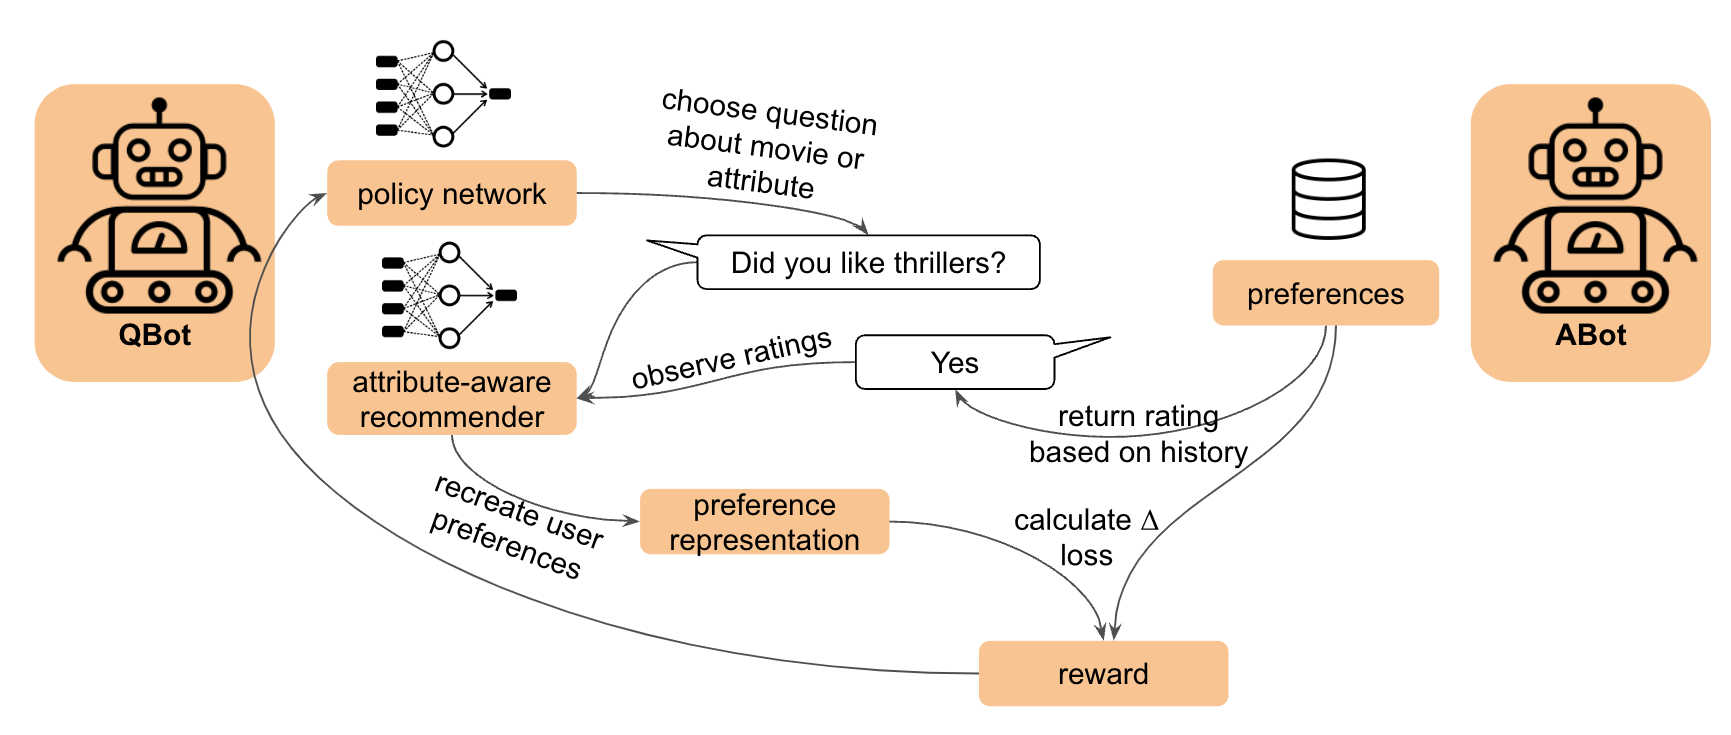
\includegraphics[scale=0.25]{figures/system_architecture.png}
    \caption{Attribute-based Conversational Recommender System architecture}
    \label{fig:system_architecture}
\end{figure}

The key components of the system are: 
\begin{enumerate}
    \item \textit{QBot}, whose goal is to proactively elicit preference information from \textit{ABot} by asking about movie ratings in order to maximise recommendation quality
    \item \textit{ABot}, which acts deterministically by retrieving the item and attribute preferences from user’s history in response to \textit{QBot}’s question
    \item \textit{Recommendation network} $\phi$, which predicts movie ratings based on the observed preferences of \textit{ABot}
    \item \textit{Policy network} $\pi$, which guides the behaviour of \textit{QBot} and is optimised stochastically using the $\epsilon$-greedy \textit{REINFORCE} algorithm in the process of bot-play and is rewarded for providing good quality recommendations, defined as decrease is loss of the recommendation network $\phi$
\end{enumerate}

A collaborative data matrix filled with ratings is made available to the QBot in order to pre-train the Recommendation component. A vector of ratings for an additional user (not included in the matrix) is visible only to the ABot. 

ABot’s action set is comprised of possible questions, including movie titles and attribute names. A recent study of natural human conversations about movie preferences revealed that besides sharing a couple of examples of movies that they liked or disliked, humans rely heavily on generalisations and descriptions of movie attributes \citep{radlinski2019coached}. Furthermore, eliciting information about individual movie titles is extremely inefficient, considering that most users have never interacted with the majority of items. For instance, the MovieLens dataset \citep{harper2015movielens} includes 9066 distinct movies, while a median user in that dataset has only provided ratings for 71 movies, which constitutes mere 0.8\%. Therefore, it is crucial to extend the framework in order to introduce item attributes (movie metadata) alongside the items (movie IDs) into all of the individual system components to enable QBot to elicit preference information efficiently.

During the dialogue, QBot requests information about specific movie titles and attributes from the ABot's ‘history’ (vector of movie ratings), and ABot responds with a rating. Following that, QBot updates its internal representation of the ABot’s ratings for all movies based on the conversation history and collaborative data matrix. The change in the recommendation model loss in QBot's internal representation is used as a reward to train the QBot's Policy model.


\section{Methodology}

I propose to extend the existing body of conversational recommender research by leaning on the VisDial framework introduce by \cite{das2017learning} and training the policy network through a goal-driven self-supervised bot-play. Training protocol that has been originally designed for image description can be applied to the recommendation scenario with some modifications. 

For the initial set of experiments, I will focus on the reinforcement learning component, in line with the experiments reported by the original authors \cite{kottur2017natural}. The absence of supervised pre-training necessitates the use of small artificial vocabularies, so generation of natural language sentences is out of the scope here. In contrast to the VisDial approach, only the Questioner agent (QBot) is trained. The Answerer agent (ABot) is implemented as a simple deterministic algorithm that returns a movie rating from a user's history if the rating is known or a phrase 'haven't seen' if the rating is unknown.

At first, a \textit{recommendation} module is trained, which serves the same purpose as a feature regression network in VisDial experiments \citep{das2017learning}. The between-timestep difference in loss of the \textit{recommendation} network is seen as a proxy to information gain and is used in the overall architecture to calculate the reward observed by the \textit{policy} network $\pi$.

Following this, the \textit{policy} network $\pi$ is optimised stochastically using the REINFORCE algorithm in the process of bot-play. The policy network guides the behaviour of the Questioner bot, while Answerer acts deterministically. The \textit{policy} network is a feedforward neural net, which receives the following inputs: 

\begin{enumerate}
    \item movie ratings known before the current timestep (where movie indexes are positionally encoded), which represent the state $s_{t-1}$
    \item index of the movie that the Questioner asked about $a_t$
\end{enumerate}

The model is optimised using the observed reward $r_t$, operationalised as the reduction of the \textit{recommendation} network loss $\Delta L_{rec}$. The \textit{policy} network learns to predict distribution over movies that Questioner asks about (Questioner’s action space $A$, which can also be seen as its vocabulary) through maximising REINFORCE value function: $maxJ(\Theta_{policy})$, where

\begin{equation} 
\label{eq:policy_loss}
J(\Theta_{policy})=E[\log\pi_{\Theta}(a_t\vert s_{t-1})r_t]
\end{equation}

The REINFORCE algorithm maximises the product of the log-likelihood of the selected action $a_t$ and the reward $r_t$, thus pushing up the probabilities of the actions associated with the highest expected rewards. Therefore, the \textit{policy} network $\pi(a_t, r_t, s_{t-1})$ learns to assign higher probabilities to movie indexes, obtaining whose ratings will be associated with higher information gain.

The Questioner’s policy network is optimised stochastically through bot-play using an $\epsilon$-greedy algorithm. The bot-play itself is implemented using ParlAI framework for training dialogue models \citep{miller2017parlai}. Firstly, the vector of the user’s movie ratings $V_u$ is transformed in accordance to agent vocabularies. Answerer’s vocabulary consists of three phrases (‘liked’, ‘disliked’ and ‘haven’t seen’), while Questioner’s vocabulary consists of the list of available movie titles $A$. At the initialisation of the dialogue, Answerer observes a rating history of a random user $V_u$ (drawn from the dataset). Questioner is blinded to this information. At each conversational turn, Questioner utters a movie title $a_t$, drawn from the set of movie titles according to the \textit{policy} network $\pi(a_t \vert s_{t-1})$. The Answerer observes the question and utters the rating of the movie $v_t$ deterministically, based on the user’s history $V_u$. The Questioner observes its own utterance, as well as the response of the Answerer and appends the information to its internal representation of Answerer’s rating history $s_{t-1}$. Following that, the \textit{recommendation} network $\phi$ is used to compute the loss $L(s_t)$ given the observed history of ratings. The change of the said loss compared to previous conversational turn is used as a reward $r_t = \Delta L$  to optimise the weights of Questioner’s \textit{policy} network $\Theta_{\pi}$. The pseudocode is provided below.

\begin{algorithm}
    \caption{Bot-Play Training Procedure}
    \label{algo:algo_bot_play}
    \begin{algorithmic}[1]
        \Require{user $u_i$, movies $A$, ratings $V$, number of conversational rounds $T$, exploration probability $\epsilon$, recommendation function $\phi$}
        \Ensure{policy network $\pi$ parameters $\Theta$}
        \Statex
        \State {Randomly initialise policy network $\pi$ parameters $\Theta$}
        \For {$t = 1, 2, \ldots, T$}
        \State {generate probability distribution over actions $p(A \vert s_{t-1}) = \pi(s_{t-1})$}
        \If {$\epsilon >$ uniformRandom(0,1)}
        \State {question $a_t$ = randomChoice($A$)}
        \Else 
        \State {question $a_t$ = randomChoice($A$, $p(A \vert s_{t-1})$)}
        \EndIf
        \State {QBot utters $a_t$}
        \State {ABot observes $a_t$}
        \State {ABot utters rating $v_a$}
        \State {QBot observes ($a_t$, $v_a$) and updates state $s_t = s_{t-1} \cup  (a_t, v_a)$}
        \State {compute predicted ratings $\widehat{V}_t = \phi(s_t)$}
        \State {compute CE loss $L_t=-V_t\log(\widehat{V}_t)-(1-V_t)log(1-\widehat{V}_t)$}
        \State {compute reward $r_t=L_{t-1}-L_t$}
        \State {compute REINFORCE value functions $J_t=E[\log\pi(a_t\vert s_{t-1})r_t]$}
        \State {update $\Theta_{t}=\Theta_{t-1} - \nabla \log \pi_{\Theta}(a_t\vert s_{t-1})r_t$}
        \EndFor
        \State \Return {$\Theta$}
    \end{algorithmic}
\end{algorithm}


\clearpage
\section{Results}
\subsection{Policy Network Performance}
We have previously defined the main success criterion of the Questioner’s policy as learning an effective questioning strategy that would allow to uncover as much information as possible about the user in the smallest possible number of conversational turns. Therefore, we expect that the policy network will learn which questions would be the most impactful given the current state (already observed history), so as to minimise the loss of the recommendation network at each conversational turn.

As seen in Figure~\ref{fig:policy_synt}, on a synthetic dataset, the policy network has generally learned to recreate the full vector of user’s rating in five conversation turns, which corresponds to five uncorrelated movie clusters. In contrast, a random policy does not consistently achieve zero loss even in 10 conversational turns. 

\begin{figure}[ht]
    \centering
    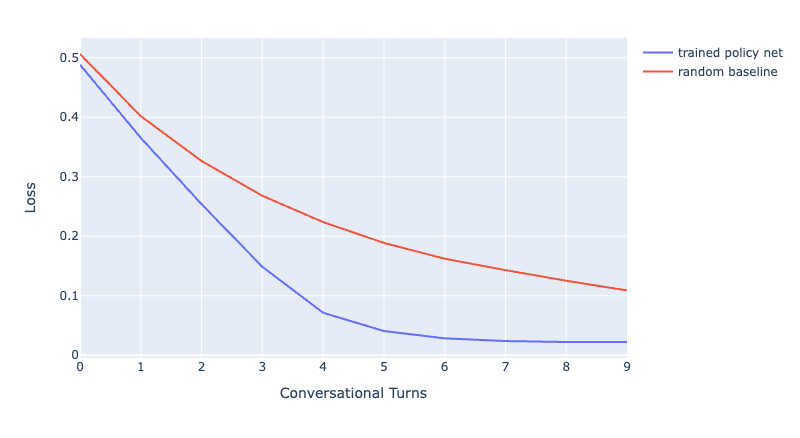
\includegraphics[scale=0.5]{figures/policy_synt.png}
    \caption{Loss decrease over conversational turns in bot-play on the synthetic dataset.}
    \label{fig:policy_synt}
\end{figure}


\clearpage
On the MovieLens-based dataset (Figure~\ref{fig:policy_movielens}), the policy network has learned to significantly reduce loss in the initial conversational turns by asking questions that are most predictive of the full rating vector. However, in contrast with the synthetic dataset, this effect diminishes over conversational turns, which is likely related to the fact that correlations between individual items in the MovieLens based dataset are much weaker than in the synthetic dataset (see Figure~\ref{fig:sw_corr}) and it is not possible to accurately recreate the full set of user's ratings from a small subset of ratings.

\begin{figure}[ht]
    \centering
    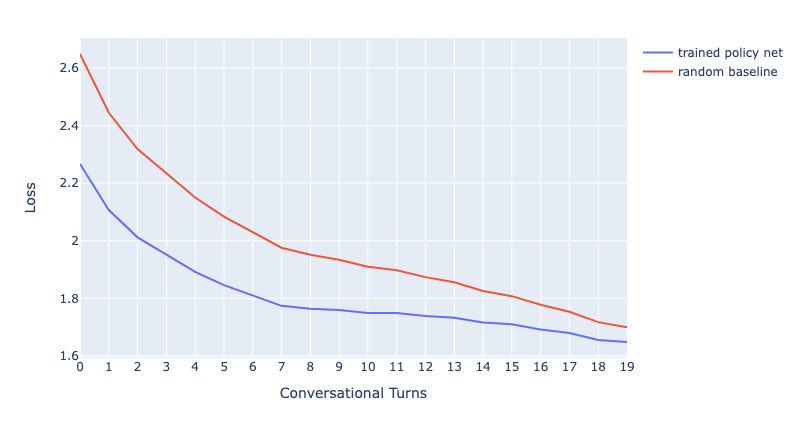
\includegraphics[scale=0.5]{figures/policy_movielens.png}
    \caption{Loss decrease over conversational turns in bot-play on the MovieLens dataset.}
    \label{fig:policy_movielens}
\end{figure}
